\documentclass[border=10pt]{standalone}

\usepackage{tikz}
\usepackage{tikzsymbols}
\usetikzlibrary{calc,patterns,shapes.geometric}

\def\centerarc[#1](#2)(#3:#4:#5){\draw[#1] ($(#2)+({#5*cos(#3)},{#5*sin(#3)})$) arc (#3:#4:#5);}

\begin{document}
	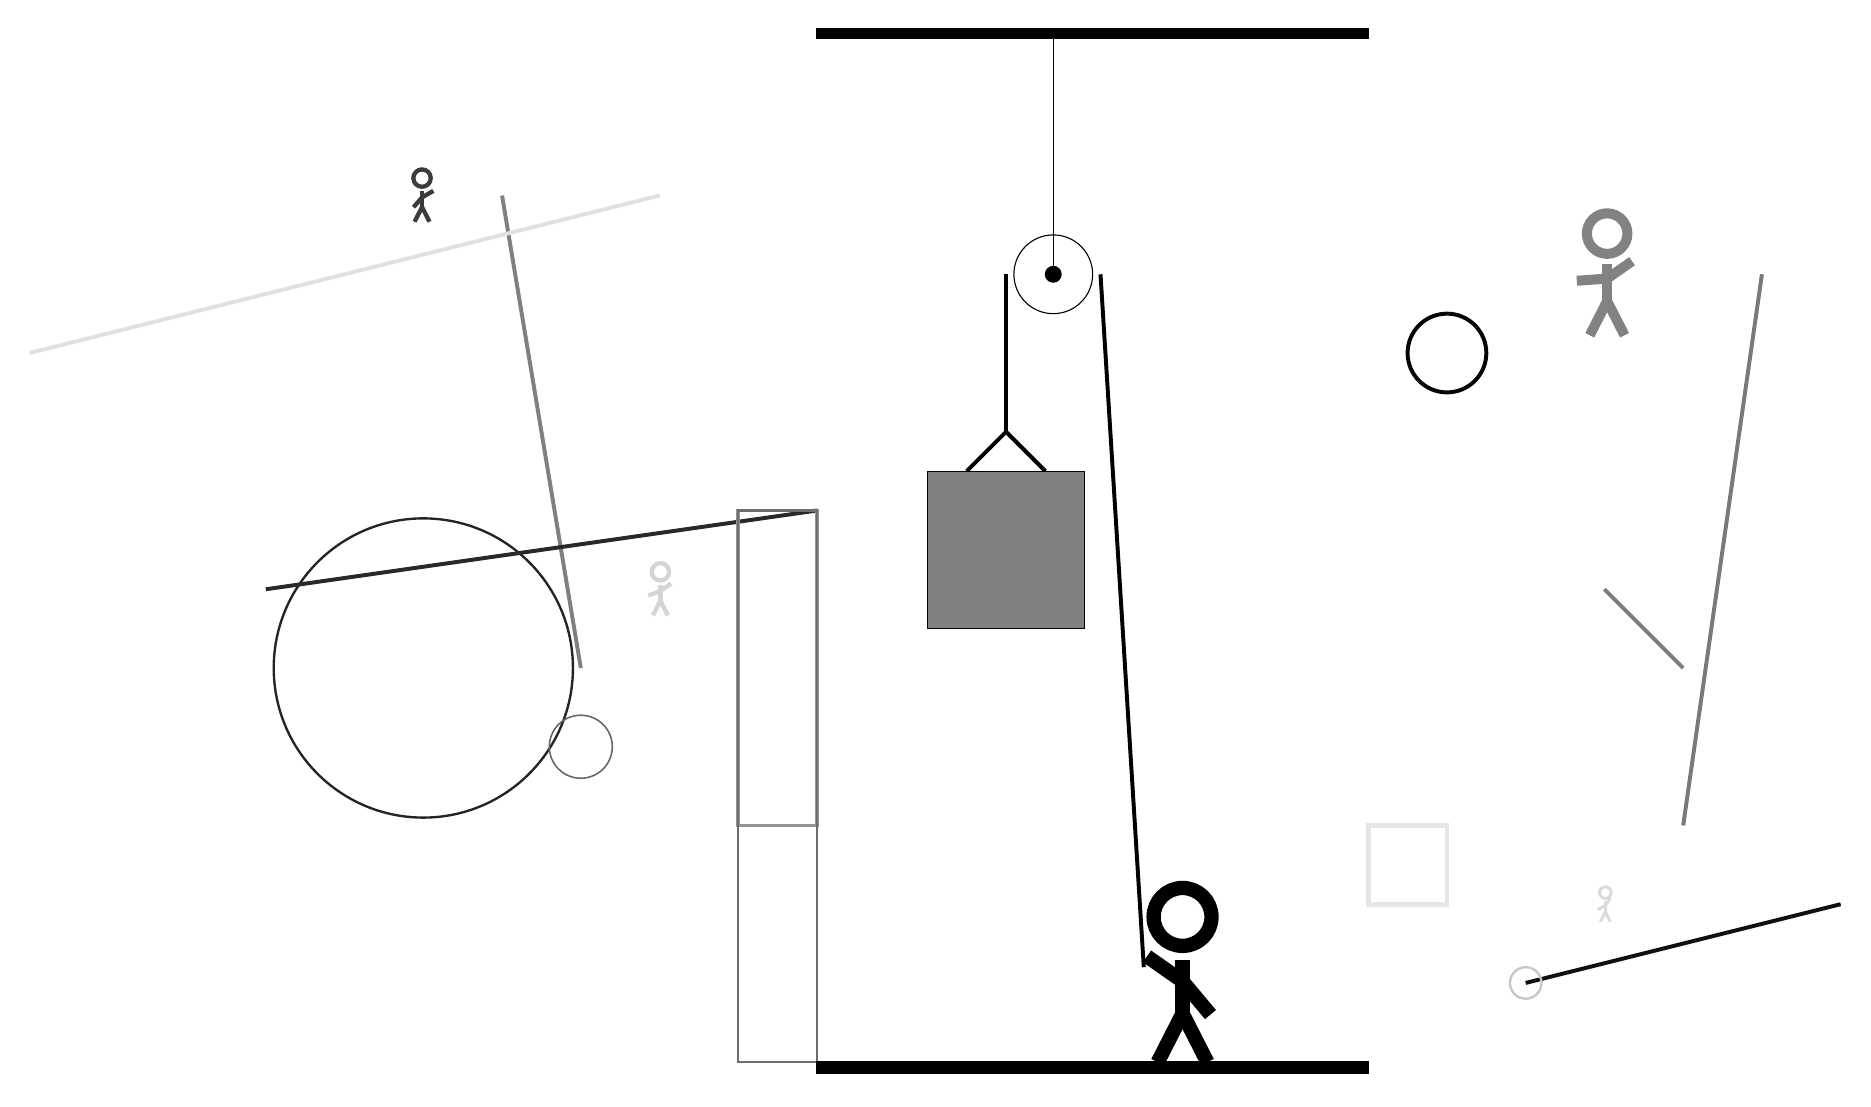
\begin{tikzpicture}
		%%%%% START %%%%%
		
		\draw[fill=black] (-2, 10) rectangle (5, 10.125);
		
		\draw (1, 7) circle (0.5);
		\draw[fill=black] (1, 7) circle (0.1);
		\draw (1, 10) -- (1, 7);
		
		\draw[line width=0.5mm] (-0.1, 4.5) -- (0.4, 5.0) -- (0.9, 4.5);
		\draw[fill=black!50] (-0.6, 4.5) rectangle (1.4, 2.5);
		
		\draw [line width=0.5mm, color=black!98](6, 6) circle (0.5);
		
		\draw [line width=0.3mm, color=black!86](-7, 2) circle (1.9);
		\draw[line width=0.5mm, color=black!50](-5, 2) -- (-6, 8);
		\draw[line width=0.5mm, color=black!84](-2, 4) -- (-9, 3);
		\node[line width=0.2mm, color=black!77] at (-7, 8) {\Strichmaxerl[3][49][30]};
		\draw [line width=0.6mm, color=black!78](7, 5) circle (0.0);
		
		\draw[line width=0.6mm, color=black!10] (5, 0) rectangle (6, -1);
		
		\draw[line width=0.5mm, color=black!94](7, -2) -- (11, -1);
		\node[line width=0.2mm, color=black!49] at (8, 7) {\Strichmaxerl[7][4][35]};
		\draw [line width=0.3mm, color=black!22](7, -2) circle (0.2);
		\draw[line width=0.5mm, color=black!52](9, 0) -- (10, 7);
		\node[line width=0.3mm, color=black!15] at (8, -1) {\Strichmaxerl[2][29][55]};
		\draw [line width=0.2mm, color=black!60](-5, 1) circle (0.4);
		
		\node[line width=0.5mm, color=black!17] at (-4, 3) {\Strichmaxerl[3][20][36]};
		\draw[line width=0.5mm, color=black!42] (-2, 0) rectangle (-3, 4);
		\draw[line width=0.5mm, color=black!51](8, 3) -- (9, 2);
		
		\draw[line width=0.5mm, color=black!12](-4, 8) -- (-12, 6);
		
		\draw[line width=0.3mm, color=black!57] (-3, 4) rectangle (-2, -3);
		
		\draw[line width=0.5mm] (0.4, 7) -- (0.4, 5.0);
		\centerarc[line width=0.5mm](1, 7)(0:180:0.6);
		\draw[line width=0.5mm](1.6, 7) -- (2.15, -1.8);
		
		\node at (2.6, -1.9) {\Strichmaxerl[10][-35][-50]};
		
		\draw[fill=black] (-2, -3) rectangle (5, -3.15);
		
		%%%%% END %%%%%
	\end{tikzpicture}
\end{document}